\documentclass[11pt,a4paper]{article}
\usepackage{amsmath}
\usepackage{amsfonts}
\usepackage{tikz,pgfplots}
\usepackage{gensymb}
\usepackage{graphicx}

\usepackage{epstopdf}
%\usepackage{listings}
\usepackage{tikz,fp,fp-random,todonotes}
\usepackage[procnames]{listings}
\usepackage{afterpage}
%\usepackage[margin=1in]{geometry}
\usepackage{titlesec}
\usepackage{float}
\usepackage{amsthm}
\usepackage{wrapfig}
\usepackage{booktabs,caption}
\usepackage[flushleft]{threeparttable}
\usepackage{scrextend}
\usepackage{stfloats}
\usepackage{mathtools}
\usepackage{bm}
\usepackage{stackengine}
\usepackage[hidelinks]{hyperref}
\usepackage{siunitx}
\usepackage{subfig}
\usepackage{authblk}
\usepackage[margin=0.7in]{geometry}
 
\addtokomafont{labelinglabel}{\sffamily}


\usetikzlibrary{calc}
\usetikzlibrary{backgrounds}
\usetikzlibrary{calc}
\usetikzlibrary{decorations.markings}
\usetikzlibrary{arrows}
\usetikzlibrary{positioning}
\usetikzlibrary{decorations.text}

\usetikzlibrary{shadings}
\usetikzlibrary{backgrounds}
\usetikzlibrary{calc}
\usetikzlibrary{decorations.markings}
\usetikzlibrary{arrows}
\usetikzlibrary{positioning}
\usetikzlibrary{decorations.text}
\usetikzlibrary{shapes.multipart}
        
\allowdisplaybreaks
\renewcommand{\floatpagefraction}{.85}

\newcommand{\x}{{\bf x}}
\renewcommand{\d}{{\rm d}}
\newcommand{\e}{{\rm e}}
\newcommand{\ii}{{\rm i}}

\newcommand{\tmi}{\tau_0\wedge\tau}
\newcommand{\tma}{\tau_0\vee\tau}
\newcommand{\taua}{\tau_{\rm A}}


\begin{document}
\title{Modeling the effect of aneuploidy on cancer evolution}
\author[1]{Remus Stana}
\author[2]{Daniel Weissman}
\author[1]{Yoav Ram}
\affil[1]{School of Zoology, Tel Aviv University, Tel Aviv-Yafo, Israel}
\affil[2]{Department of Physics, Emory University, Atlanta, United States of America}

\maketitle

\begin{abstract}
Evolutionary rescue is the process by which a population is able to survive a sudden environmental change which initially causes the population to decline towards extinction. A prime example of evolutionary rescue is the ability of cancer to survive being exposed to various treatments. We are interested in the mechanisms through which a population of cancer cells are able to adapt to chemotherapy, and in particular, the role played by chromosomal instability (aneuploidy). Cancer cells which have aneuploidy are hypothesized to have a higher fitness in an environment altered by anti-cancer drugs as they have incomplete pathways which drugs activate in order to kill the cells. Aneuploidy is highly prevalent in tumors and certain drugs which attempt to combat cancers through increasing chromosomal instability. As a result, the question we wish to answer is how aneuploidy impacts the fate of the population of cancer cells. We propose to model evolutionary rescue with the help of multi-type branching processes to obtain the probability that cancer will survive. Additionally, we will utilize large genomic datasets to asses the effects of aneuploidy on the probability of evolutionary rescue.
\end{abstract}

\section{Introduction}
%The question of what role does chromosomal instability (CIN) play in the emergence of cancer has been studied extensively in the past decades \cite{michor2005can,christine2018understanding,nowak2002role,pavelka2010dr,komarova2003mutation,zhu2018cellular}. One hypothesis is that CIN facilitates tumorgenesis by accelerating the removal of tumor suppression genes (TSG) and subsequent appearance of cancer. The deletion of tumor suppression genes can happen in two ways (see Figure \ref{figureCIN}): two point mutations deleting both alleles of the TSG or one point mutation and one chromosomal loss event. The case of two chromosomal loss events is taken into consideration because the fitness cost would be very large and the cell would die.
%
%Populations adapted to a certain environment are vulnerable to change in the environment which might cause extinction of the population. Adaptation is a race against time as the population size decreases in the new environment. Evolutionary rescue is the process where the population acquires mutations which increases the fitness of the population in the new environment such that the extinction in averted. We are interested in how likely is a population to adapt to the changing environment through evolution. Examples of such changes include climate change, invasive species or the onset of drug therapies. There exists three possible ways for a population to survive environmental degradation: migration to a new habitat similar to the one before the onset of environmental changes \cite{cobbold2020should}, adaptation by phenotypic plasticity which involves no changes in the genotype\cite{carja2019evolutionary,carja2017evolutionary} and adaptation through genetic mutations\cite{uecker2014evolutionary,uecker2016role,uecker2011fixation}.
%
%Majority of studies assume that the fitness of the wildtype and mutant are time homogeneous. An exception is \cite{marrec2020adapt} fitness of wildtype and mutant are taken to be functions of time.

%%%%%%

Populations adapted to a certain environment are vulnerable to environmental changes, which might cause extinction of the population. Examples of such environmental changes include climate change, invasive species or the onset of drug therapies. Adaptation is a race against time as the population size decreases in the new environment\cite{tanaka2022surviving}. 
{\em Evolutionary rescue} is the process where the population acquires mutations that increase the fitness of the population in the new environment such that extinction is averted. It is mathematically equivalent to the problem of crossing of fitness valley \cite{weissman2009rate,weissman2010rate}.
We are interested in how likely is a population to adapt to the changing environment through evolutionary adaptation.
There are three potential ways for a population to survive environmental degradation: migration to a new habitat similar to the one before the onset of environmental change \cite{cobbold2020should}; adaptation by phenotypic plasticity without genetic change \cite{carja2019evolutionary,carja2017evolutionary,levien2021non}; and adaptation through genetic mutations \cite{uecker2014evolutionary,uecker2016role,uecker2011fixation}.

Chromosomal instability (CIN) is the process during mitosis in which cells suffer from chromosome segration defects, which leads to a state called aneuploidy where cells are characterized by structural changes of the chromosomes and copy number alterations \cite{schukken2018cin}.

Aberrations in chromosome copy number are exploited by cancer cells in order to survive under conditions of selective pressure such as chemotherapy. % REF
Cancer cells are likely to be aneuploid, which also correlates with poor patient outcomes \cite{ben2020context}. One mechanism by which aneuploidy has been hypothesized to rescue cancer is by providing phenotypic variation and increasing heterogeneity in a tumor. 

The role of chromosomal instability (CIN) in the emergence of cancer has been studied extensively in the past decades \cite{michor2005can,christine2018understanding,nowak2002role,pavelka2010dr,komarova2003mutation,zhu2018cellular}.
One hypothesis is that CIN facilitates tumor genesis by accelerating the removal of tumor suppression genes (TSG) and subsequent appearance of cancer. The deletion of tumor suppression genes can happen in two ways: two point mutations deleting both alleles of the TSG (assuming a diploid genotype), or one point mutation and one chromosomal loss event. Initial studies have shown that aneuploidy can have a significant role in the deletion of the the tumor suppressing genes when compared to two consecutive point mutations\cite{nowak2002role,komarova2003mutation,michor2005can,komarova2008selective}. % REF ok
However, when taking into account that the appearance of aneuploidy requires a mutation to trigger chromosomal instability, the probability that CIN precedes tumor genesis is highly unlikely.

Majority of studies assume that the fitness of the wildtype and mutant are independent of time. An exception is \cite{marrec2020adapt}, where the fitness of the wildtype and mutant are time dependent. Additionally, \cite{uecker2011fixation} investigated the probability of fixation of a beneficial mutation in a variable environment with arbitrary time-dependent selection coefficient and population size.

Most studies on evolutionary rescue are interested in the probability that at least one mutation rescues the population but the question of wheter multiple mutations contribute to the survival of the population is less explored. One exception is \cite{wilson2017soft} which show that evolutionary rescue is significantly inhanced by soft selective sweeps when multiple mutations contribute. 

Evolutionary rescue which requires two succesive mutations has been investigated by \cite{martin2013probability} with the help of diffusion approximation.

\begin{figure}
\centering
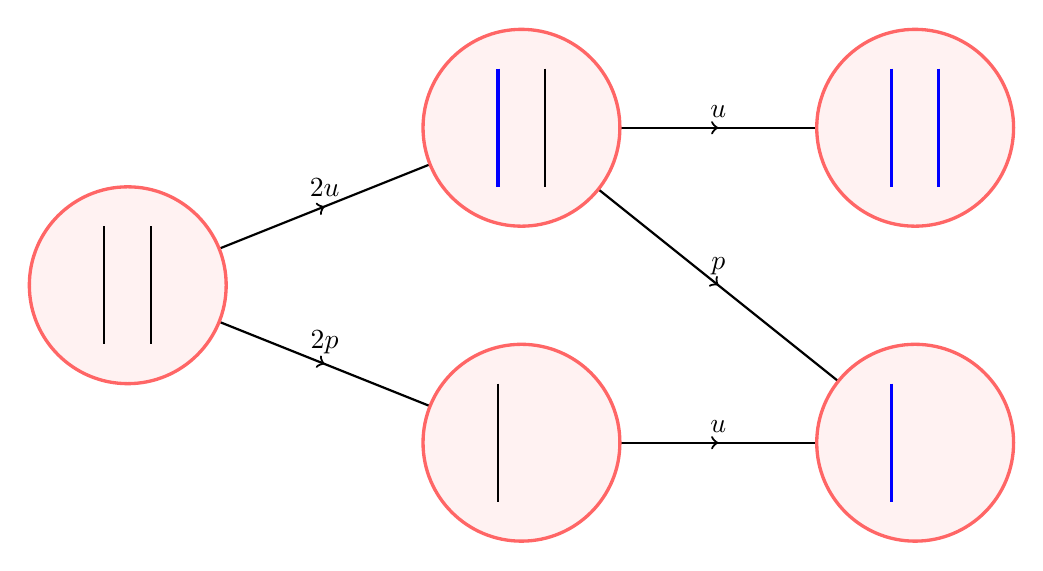
\begin{tikzpicture}[very thick,decoration={
    markings,
    mark=at position 0.5 with {\arrow{>}}}
    ] 
\edef\x{6.5} 
\edef\y{-0.5} 
\edef\r{1.25} 

\draw [postaction={decorate}, thick](-0.25,-2) -- (-0.25+5,0) node [midway, above] {$2u$};
\draw [postaction={decorate}, thick](-0.25,-2) -- (-0.25+5,-4) node [midway, above] {$2p$};
\draw [postaction={decorate}, thick](-0.25+5+\r,-0) -- (-0.25+10-\r,-0) node [midway, above] {$u$};
\draw [postaction={decorate}, thick](-0.25+5+\r,-4) -- (-0.25+10-\r,-4) node [midway, above] {$u$};
\draw [postaction={decorate}, thick](-0.25+5,-0) -- (-0.25+10,-4) node [midway, above] {$p$};

\filldraw[color=red!60, fill=red!5, very thick](-0.25,-2) circle (\r);
\filldraw[color=red!60, fill=red!5, very thick](-0.25+5,0) circle (\r);
\filldraw[color=red!60, fill=red!5, very thick](-0.25+5,-4) circle (\r);
\filldraw[color=red!60, fill=red!5, very thick](-0.25+10,0) circle (\r);
\filldraw[color=red!60, fill=red!5, very thick](-0.25+10,-4) circle (\r);

\draw [thick](0.05,-1.25) -- (0.05,-2.75);
\draw [thick](-0.55,-1.25) -- (-0.55,-2.75);

\draw [thick](0.05+5,-1.25+2) -- (0.05+5,-2.75+2);
\draw [very thick, blue](-0.55+5,-1.25+2) -- (-0.55+5,-2.75+2);

\draw [very thick, blue](0.05+10,-1.25+2) -- (0.05+10,-2.75+2);
\draw [very thick, blue](-0.55+10,-1.25+2) -- (-0.55+10,-2.75+2);

\draw [thick](-0.55+5,-1.25-2) -- (-0.55+5,-2.75-2);

\draw [very thick, blue](-0.55+10,-1.25-2) -- (-0.55+10,-2.75-2);
\end{tikzpicture}
\caption{Diagram of tumorgenesis by which a cell loses both of its tumor suppressing cells. The first tumor suppressing gene can be eliminated by a mutation at rate $2u$ or through chromosomal instability with rate $2p$. The last TSG can either be eliminated through mutation at rate $u$ or through chromosomal instability with rate $p$. Grey vertical lines represent active TSGs while the blue vertical lines represent inactivated TSGs.
}
\label{figureCIN}
\end{figure}

%%%%%%%%%%%%%%%%%%%%%%%%%%%%%%%%%%%%%%%%%%%%%%%%%%%%%%%%%%%%%%%%%

\begin{figure}
\centering
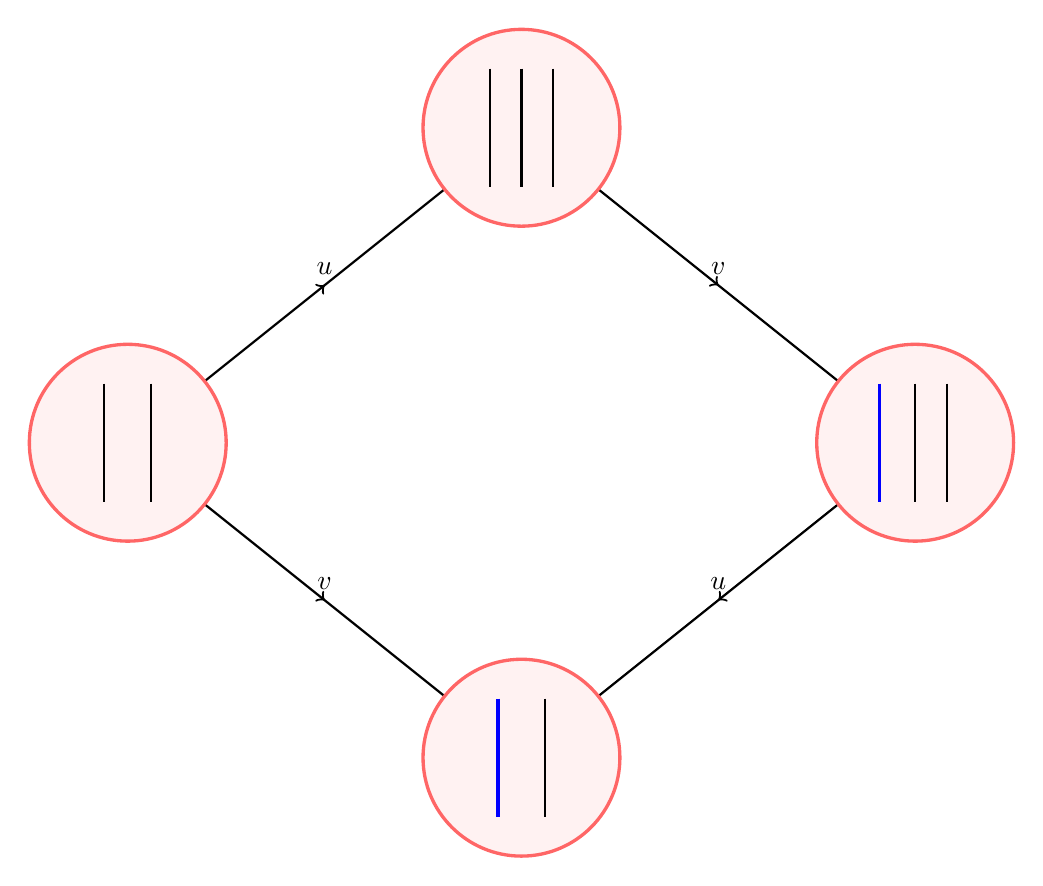
\begin{tikzpicture}[very thick,decoration={
    markings,
    mark=at position 0.5 with {\arrow{>}}}
    ] 
\edef\x{6.5} 
\edef\y{-0.5} 
\edef\r{1.25} 

\draw [postaction={decorate}, thick](-0.25,-4) -- (-0.25+5,0) node [midway, above] {$u$};
%\draw [postaction={decorate}, thick](-0.25,-2) -- (-0.25+5,-4) node [midway, above] {$2p$};
\draw [postaction={decorate}, thick](-0.25+5,-0) -- (-0.25+10,-4) node [midway, above] {$v$};
%\draw [postaction={decorate}, thick](-0.25+5+\r,-4) -- (-0.25+10-\r,-4) node [midway, above] {$u$};
%\draw [postaction={decorate}, thick](-0.25+5,-0) -- (-0.25+10,-4) node [midway, above] {$p$};
\draw [postaction={decorate}, thick]  (-0.25+10,-4) -- (-0.25+5,-8) node [midway, above] {$u$};
\draw [postaction={decorate}, thick](-0.25,-4)  -- (-0.25+5,-8)  node [midway, above] {$v$};

\filldraw[color=red!60, fill=red!5, very thick](-0.25,-4) circle (\r);
\filldraw[color=red!60, fill=red!5, very thick](-0.25+5,0) circle (\r);
%\filldraw[color=red!60, fill=red!5, very thick](-0.25+5,-4) circle (\r);
\filldraw[color=red!60, fill=red!5, very thick](-0.25+10,-4) circle (\r);
%\filldraw[color=red!60, fill=red!5, very thick](-0.25+10,-4) circle (\r);
\filldraw[color=red!60, fill=red!5, very thick](-0.25+5,-8) circle (\r);

\draw [thick](0.05,-1.25+2-4) -- (0.05,-2.75+2-4);
\draw [thick](-0.55,-1.25+2-4) -- (-0.55,-2.75+2-4);

\draw [thick](0.15+5,-1.25+2) -- (0.15+5,-2.75+2);
\draw [thick](-0.65+5,-1.25+2) -- (-0.65+5,-2.75+2);
\draw [thick](-0.25+5,-1.25+2) -- (-0.25+5,-2.75+2);

\draw [thick](0.15+10,-1.25+2-4) -- (0.15+10,-2.75+2-4);
\draw [thick](-0.25+10,-1.25+2-4) -- (-0.25+10,-2.75+2-4);
\draw [color=blue,very thick](-0.7+10,-1.25+2-4) -- (-0.7+10,-2.75+2-4);

\draw [thick](0.05+5,-1.25+2-8) -- (0.05+5,-2.75+2-8);
\draw [color=blue,very thick](-0.55+5,-1.25+2-8) -- (-0.55+5,-2.75+2-8);
%\draw [thick](-0.55+5,-1.25-2) -- (-0.55+5,-2.75-2);

%\draw [thick](-0.55+10,-1.25-2) -- (-0.55+10,-2.75-2);
\end{tikzpicture}
\caption{Diagram of the evolutionary rescue process which involves aneuploidy. The wildtype cell can either acquire trisomy at rate $u$ or aquire a fitness increasing mutation at rate $v$. Aneuploidy cells can  aquire a fitness increasing mutation at rate $v$. Finally, the aneuploidy cells can lose trisomy at rate $u$.
}
\label{figuretrisomy}
\end{figure}

\section{Model}
We model evolutionary rescue of cancer cells through aneuploidy with the help of multitype branching processes: we have three populations of cancer cells, wildtype euploid $w_t$, wildtype aneuploid $a_t$ and mutant euploid cells $m_t$ which proliferate and die with rates $\lambda_w,  \lambda_a,  \lambda_m$ and $\mu_w, \mu_a, \mu_m$, respectively. Wildtype cells can acquire aneuploidy at rate $u$ while aneuploidy and wildtype cells can mutate with rate $v$ (se Figure \ref{figureAneuploidy}). Changes in the number of wildtype euploid, wildtype aneuploid and mutant euploid cells occur at rates:
\begin{subequations}
\begin{flalign}
w_t&\rightarrow w_t+1:\quad \lambda_ww_t,\\
w_t&\rightarrow w_t-1:\quad \left(\mu_w+u+v\right)w_t,\\
a_t&\rightarrow a_t+1:\quad \lambda_aa_t+uw_t,\\
a_t&\rightarrow a_t-1:\quad \left(\mu_a+v\right)a_t,\\
m_t&\rightarrow m_t+1:\quad \lambda_am_t+va_t+vm_t,\\
m_t&\rightarrow m_t-1:\quad \mu_am_t.
\end{flalign}
\end{subequations}
Given that we have used branching processes, the lineages produced by cells from the initial population will be independent of each other. This is not a biologically realistic model as cells compete for resources in tumors. We will study a more biologically realistic model in Section.
The survival probability of a population consisting initially of one wildtype cell satisfies the quadratic equation:
\begin{align}\nonumber
1-p_w&=\frac{\mu_w}{\lambda_w+\mu_w+u+v}+\frac{u}{\lambda_w+\mu_w+u+v}\left(1-p_a\right)+\frac{\lambda_w}{\lambda_w+\mu_w+u+v}\left(1-p_w\right)^2\\ \label{quadraticeqev1}
&+\frac{v}{\lambda_w+\mu_w+u+v}\left(1-p_m\right),
\end{align}
where the $p_a$ and $p_w$ are the survival probabilities of a population consisting initially of one aneuploidy and wildtype cell, respectively.

 The smallest solution of the quadratic equation \eqref{quadraticeqev1} gives the survival probability:
\begin{align}\label{survprobw}
p_w=\frac{\lambda_w-\mu_w-u-v+\sqrt{\left(\lambda_w-\mu_w-u-v\right)^2+4\lambda_w\left(up_a+vp_m\right)}}{2\lambda_w}.
\end{align}
If the population originally consists of a single aneuploidy cell, then the probability that the population will survive is given by the following quadratic equation:
\begin{align}
1-p_a=\frac{\mu_a}{\lambda_a+\mu_a+v}+\frac{v}{\lambda_a+\mu_a+v}\left(1-p_m\right)+\frac{\lambda_a}{\lambda_a+\mu_a+v}\left(1-p_a\right)^2,
\end{align}
whose smallest solution is the survival probability:
\begin{align}\label{survproba}
p_a=\frac{\lambda_a-\mu_a-v+\sqrt{\left(\lambda_a-\mu_a-v\right)^2+4\lambda_avp_m}}{2\lambda_a}.
\end{align}
The probability that a single mutant cell will survive is given by (see Appendix \ref{AppendixSurvLin}):
\begin{equation}
p_m=\left\{
  \begin{array}{@{}ll@{}}
  \frac{\lambda_m-\mu_m}{\lambda_m},\quad\text{if }\lambda_m>\mu_m \\
   0,\quad\text{else}.
  \end{array}\right.
  \end{equation}
%%%%%%%%%%%%%%%%%%%%%%%%%%%%%%%%%%%%%%%%%%%%%%%%%%%%%%%%%%%%
\begin{figure}
\centering
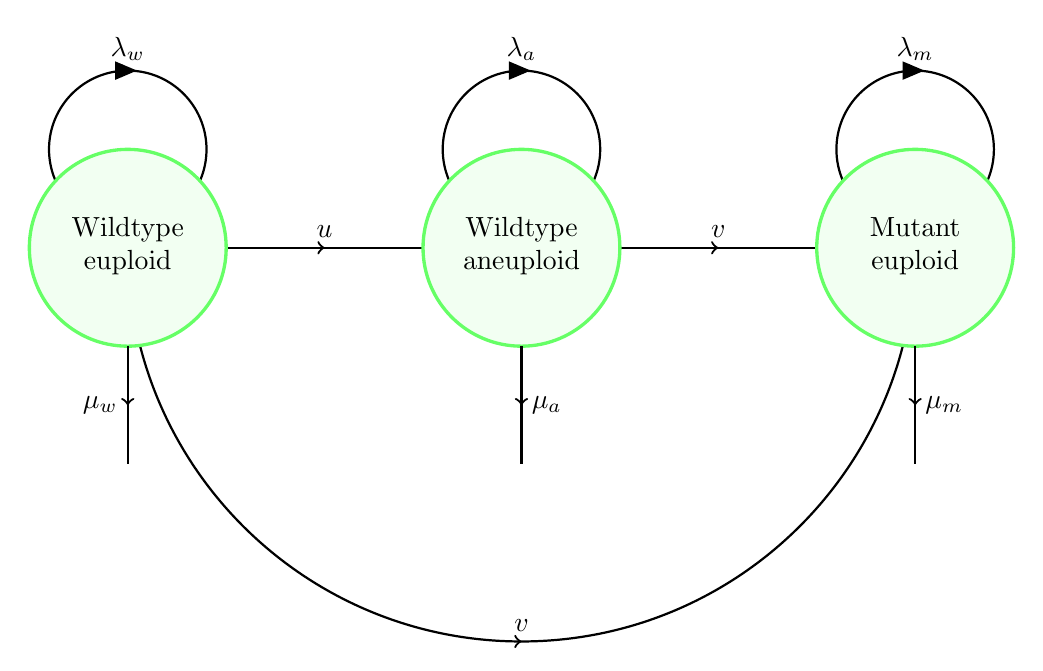
\begin{tikzpicture}[very thick,decoration={
    markings,
    mark=at position 0.5 with {\arrow{>}}}, middlearrow/.style 2 args={
        decoration={             
            markings, 
            mark=at position 0.5 with {\arrow[xshift=3.333pt]{triangle 45}, \node[#1] {#2};}
        },
        postaction={decorate}
    }]
\edef\x{6.5} 
\edef\y{-0.5} 
\edef\r{1.25} 

\edef\R{1} 
\edef\Y{0.25} 

\draw[black,thick,middlearrow={above}{$\lambda_w$},text=black] (-0.25,\Y) arc (270:-90:\R);
\draw[black,thick,middlearrow={above}{$\lambda_a$},text=black] (-0.25+5,\Y) arc (270:-90:\R);
\draw[black,thick,middlearrow={above}{$\lambda_m$},text=black] (-0.25+10,\Y) arc (270:-90:\R);

\draw [postaction={decorate}, thick](-0.25,0) -- (-0.25+5,0) node [midway, above] {$u$};
\draw [postaction={decorate}, thick](-0.25+5+\r,-0) -- (-0.25+10-\r,-0) node [midway, above] {$v$};

\draw[thick, postaction={decorate}] (-0.25,0) arc (180:360:5) node [midway, above] {$v$};


\filldraw[color=green!60, fill=green!5, very thick](-0.25,0) circle (\r);
\filldraw[color=green!60, fill=green!5, very thick](-0.25+5,0) circle (\r);
\filldraw[color=green!60, fill=green!5, very thick](-0.25+10,0) circle (\r);

\draw [thick, postaction={decorate}](-0.25,-1.25) -- (-0.25,-2.75) node [midway, left] {$\mu_w$};

\draw [thick, postaction={decorate}](-0.25+5,-1.25) -- (-0.25+5,-2.75) node [midway, right] {$\mu_a$};

\draw [thick, postaction={decorate}](-0.25+10,-1.25) -- (-0.25+10,-2.75) node [midway, right] {$\mu_m$};

\edef\x{0.25} 
\edef\y{-0.25} 

\node[text width=2cm,align=justify] at (\y,\x)  
{\begin{center}
Wildtype  euploid
\end{center}};

\node[text width=2cm,align=justify] at (\y+5,\x)  
{\begin{center}
Wildtype  aneuploid
\end{center}};

\node[text width=2cm,align=justify] at (\y+10,\x)  
{\begin{center}
Mutant  euploid
\end{center}};
\end{tikzpicture}
\caption{Diagram of the evolutionary rescue model where the population of cancer cells is subdivided to wildtype euploid, wildtype aneuploid and mutant euploid cells that divide and die with rates $\lambda_w,  \lambda_a,  \lambda_m$ and $\mu_w, \mu_a, \mu_m$, respectively. Wildtype cells can acquire aneuploidy at rate $u$. Aneuploid and wildtype cells can mutate with rate $v$.}
\label{figureAneuploidy}
\end{figure}
%%%%%%%%%%%%%%%%%%%%%%%%%%%%%%%%%%%%%%%%%%%%%%%%%%%%%%%%%%%%%

\section{First case: $4\lambda_avp_m<\left(\lambda_a-\mu_a-v\right)^2$}
\subsection{$\lambda_a>\mu_a$ and $\lambda_w<\mu_w$}
We assume that $\lambda_a>\mu_a$ and $\lambda_w<\mu_w$ and, as a result, we rewrite \eqref{survprobw} and \eqref{survproba} as:
\begin{align*}
p_a&=\frac{\lambda_a-\mu_a-v}{2\lambda_a}\left(1+\sqrt{1+\frac{4\lambda_avp_m}{\left(\lambda_a-\mu_a-v\right)^2}}\right),\\
p_w&=\frac{\lambda_w-\mu_w-u-v}{2\lambda_w}\left(1-\sqrt{1+\frac{4\lambda_w\left(vp_m+up_a\right)}{\left(\lambda_w-\mu_w-u-v\right)^2}}\right).
\end{align*}
Making use of the Taylor series expansions:
\begin{align*}
\left(1+\frac{4\lambda_avp_m}{\left(\lambda_a-\mu_a-v\right)^2}\right)^{\frac{1}{2}}&=1+\frac{2\lambda_avp_m}{\left(\lambda_a-\mu_a-v\right)^2}+\cdots\\
\left(1+\frac{4\lambda_w\left(vp_m+up_a\right)}{\left(\lambda_w-\mu_w-u-v\right)^2}\right)^{\frac{1}{2}}&=1+\frac{2\lambda_w\left(vp_m+up_a\right)}{\left(\lambda_w-\mu_w-u-v\right)^2}+\cdots
\end{align*}
we obtain the following approximation for the survival probability of a population consisting of a single individual wildtype cell:
\begin{align}\label{survprobwinitial}
p_w&\approx-\frac{vp_m+up_a}{\lambda_w-\mu_w-u-v}\\
\nonumber
&\approx-\frac{1}{\lambda_w-\mu_w-u-v}\left[\frac{v\left(\lambda_a-\mu_a-u\right)}{\lambda_a}+\frac{uv\left(\lambda_m-\mu_m\right)}{\lambda_m\left(\lambda_a-\mu_a-u\right)}+\frac{v\left(\lambda_m-\mu_m\right)}{\lambda_m}\right]\\ \label{survprobw2}
&\approx-\frac{1}{\lambda_w-\mu_w}\left[\frac{v\left(\lambda_a-\mu_a\right)}{\lambda_a}+\frac{uv\left(\lambda_m-\mu_m\right)}{\lambda_m\left(\lambda_a-\mu_a\right)}+\frac{v\left(\lambda_m-\mu_m\right)}{\lambda_m}\right],
\end{align}
where in the last line we have used the fact that $u,v\ll1$. Using the notational convention
\begin{equation}\label{notationalconv}
\Delta_i=\lambda_i-\mu_i,
\end{equation}
we write \eqref{survprobw} as
\begin{equation}\label{survprobwapprox}
p_w=-\frac{1}{\Delta_w}\left(\frac{v\Delta_a}{\lambda_a}+\frac{uv\Delta_m}{\lambda_m\Delta_a}+\frac{v\Delta_m}{\lambda_m}\right).
\end{equation}
Given an initial population consisting of $N$ wildtype cancer cells, the probability that the population will survive is given by: 
\begin{align}
p_{est}=1-\left(1-p_w\right)^N\approx 1-\e^{-Np_w}=1-\exp\left[\frac{N}{\Delta_w}\left(\frac{v\Delta_a}{\lambda_a}+\frac{uv\Delta_m}{\lambda_m\Delta_a}+\frac{v\Delta_m}{\lambda_m}\right)\right],
\end{align}
which we plot in Figure \ref{SurvPlotNData} as a function of $N$ and in Figure \ref{SurvPlot} as a function of $\lambda_w$. 

We want to improve the accuracy of our approximation by taking into consideration the second term of the Taylor series expansion:
\begin{align*}
\left(1+\frac{4\lambda_avp_m}{\left(\lambda_a-\mu_a-v\right)^2}\right)^{\frac{1}{2}}=1+\frac{2\lambda_avp_m}{\left(\lambda_a-\mu_a-v\right)^2}-\frac{\left(\lambda_avp_m\right)^2}{4\left(\lambda_a-\mu_a-v\right)^4}+\cdots,
\end{align*}
which gives us the following approximation for $p_a$:
\begin{align}
p_a=\frac{\lambda_a-\mu_a-v}{\lambda_a}+\frac{vp_m}{\lambda_a-\mu_a-v}-\frac{\lambda_a\left(vp_m\right)^2}{8\left(\lambda_a-\mu_a-v\right)^3}
\end{align}
From which we deduce that:
\begin{align}\nonumber
p_w&\approx-\frac{1}{\lambda_w-\mu_w-u-v}\left[\frac{v\left(\lambda_a-\mu_a-u\right)}{\lambda_a}+\frac{uv\left(\lambda_m-\mu_m\right)}{\lambda_m\left(\lambda_a-\mu_a-u\right)}+\frac{v\left(\lambda_m-\mu_m\right)}{\lambda_m}-\frac{uv^2\lambda_a\left(\lambda_m-\mu_m\right)^2}{8\lambda_m^2\left(\lambda_a-\mu_a-v\right)^3}\right]\\ \label{survprobw3}
&\approx-\frac{1}{\lambda_w-\mu_w}\left[\frac{v\left(\lambda_a-\mu_a\right)}{\lambda_a}+\frac{uv\left(\lambda_m-\mu_m\right)}{\lambda_m\left(\lambda_a-\mu_a\right)}+\frac{v\left(\lambda_m-\mu_m\right)}{\lambda_m}-\frac{uv^2\lambda_a\left(\lambda_m-\mu_m\right)^2}{8\lambda_m^2\left(\lambda_a-\mu_a\right)^3}\right].
\end{align}
Using the notations described in \eqref{notationalconv} we write the above equation as:
\begin{equation}\label{survprobwapproxcorrected}
p_w=-\frac{1}{\Delta_w}\left(\frac{v\Delta_a}{\lambda_a}+\frac{uv\Delta_m}{\lambda_m\Delta_a}+\frac{v\Delta_m}{\lambda_m}-\frac{uv^2\lambda_a\Delta_m^2}{8\lambda_m^2\Delta_a^3}\right).
\end{equation}
Given an initial population consisting of $N$ wildtype cancer cells, the probability that the population will survive is given by: 
\begin{align}
p_{est}=1-\left(1-p_w\right)^N\approx 1-\e^{-Np_w}=1-\exp\left[\frac{N}{\Delta_w}\left(\frac{v\Delta_a}{\lambda_a}+\frac{uv\Delta_m}{\lambda_m\Delta_a}+\frac{v\Delta_m}{\lambda_m}-\frac{uv^2\lambda_a\Delta_m^2}{8\lambda_m^2\Delta_a^3}\right)\right].
\end{align}
\subsection{$\lambda_a<\mu_a$ and $\lambda_w<\mu_w$}
We assume that $\lambda_a<\mu_a$ and $\lambda_w<\mu_w$ and, as a result, we rewrite \eqref{survprobw} and \eqref{survproba} as:
\begin{align*}
p_a&=\frac{\lambda_a-\mu_a-v}{2\lambda_a}\left(1-\sqrt{1+\frac{4\lambda_avp_m}{\left(\lambda_a-\mu_a-v\right)^2}}\right),\\
p_w&=\frac{\lambda_w-\mu_w-u-v}{2\lambda_w}\left(1-\sqrt{1+\frac{4\lambda_w\left(vp_m+up_a\right)}{\left(\lambda_w-\mu_w-u-v\right)^2}}\right).
\end{align*}
\begin{align}\label{survprobwinitial}
p_w&\approx-\frac{vp_m+up_a}{\lambda_w-\mu_w-u-v}\\
\nonumber
&\approx\frac{1}{\lambda_w-\mu_w-u-v}\left[\frac{uv\left(\lambda_m-\mu_m\right)}{\lambda_m\left(\lambda_a-\mu_a-v\right)}-\frac{v\left(\lambda_m-\mu_m\right)}{\lambda_m}\right]\\ \label{survprobw2}
&\approx\frac{v\left(\lambda_m-\mu_m\right)}{\lambda_m\left(\lambda_w-\mu_w\right)}\left[\frac{u}{\left(\lambda_a-\mu_a\right)}-1\right],
\end{align}
where in the last line we have used the fact that $u,v\ll1$. Using the notational convention
\begin{equation}\label{notationalconv}
\Delta_i=\lambda_i-\mu_i,
\end{equation}
we write \eqref{survprobw} as
\begin{equation}\label{survprobwapprox}
p_w=\frac{v\Delta_m}{\lambda_m\Delta_w}\left(\frac{u}{\Delta_a}-1\right).
\end{equation}
Given an initial population consisting of $N$ wildtype cancer cells, the probability that the population will survive is given by: 
\begin{align}\label{AneuploidyDeleteriousApprox}
p_{est}=1-\left(1-p_w\right)^N\approx 1-\e^{-Np_w}=1-\exp\left[\frac{v\Delta_mN}{\lambda_m\Delta_w}\left(1-\frac{u}{\Delta_a}\right)\right],
\end{align}

\begin{figure}[!t]
 \vspace*{1\baselineskip}
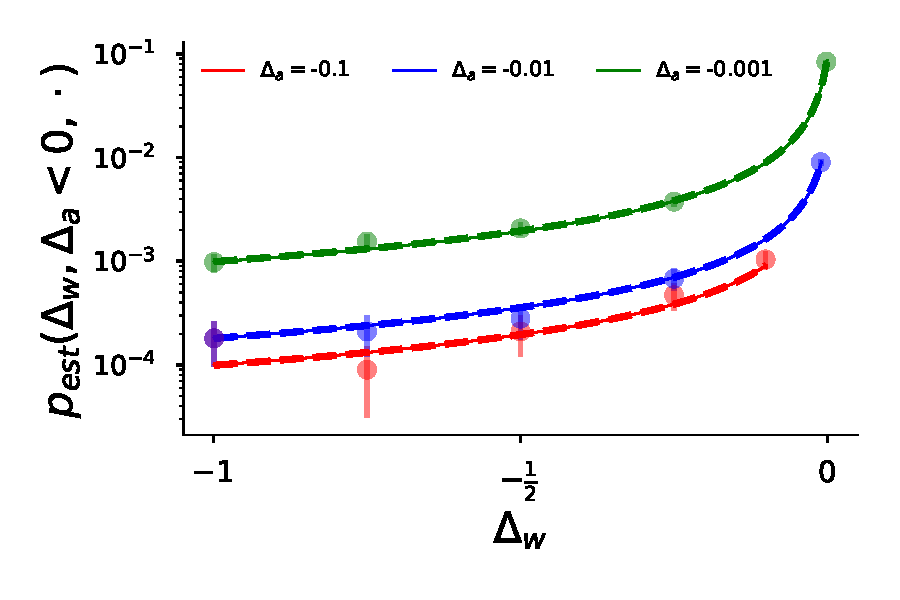
\includegraphics[width=1\textwidth]{P_est.pdf}
\caption{Plot of the survival probability of an initial population consisting of $10^{4}$ wildtype cells as a function of $\Delta_a=\lambda_a-\mu_a$ for various values of $\Delta_w=\lambda_a-\mu_a$. The continuous lines represent the exact result \eqref{survprobw} while the dashed lines represent the approximation \eqref{AneuploidyDeleteriousApprox}.}
\label{P_est}
\end{figure}
%%%%%%%%%%%%%%%%%%%%%%%%%%%%%%%%%%%%%%%%%%%%%%%%%%%%%%%%%%%%%%%%%%%%
\begin{figure}[!t]
 \vspace*{1\baselineskip}
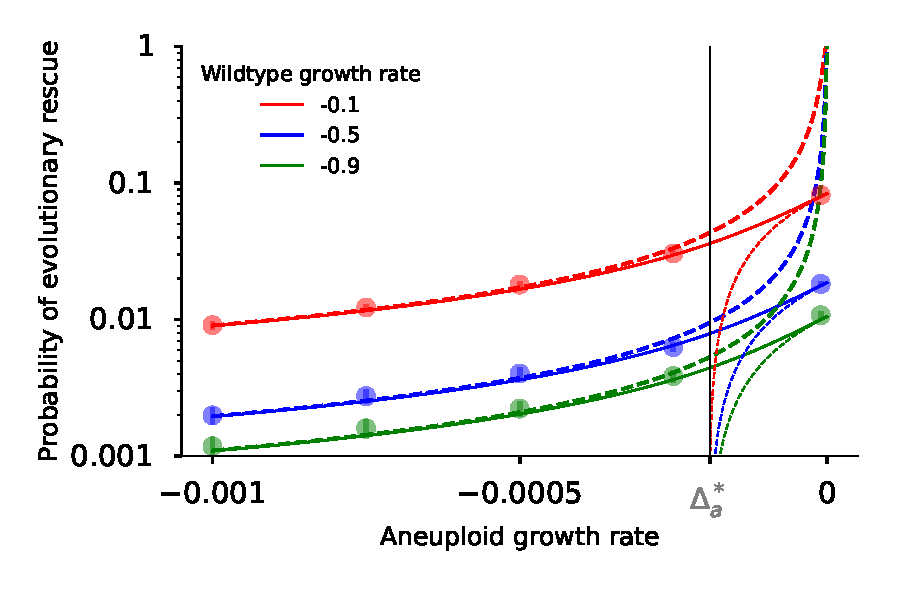
\includegraphics[width=1\textwidth]{P_est_divergence.pdf}
\caption{Plot of the survival probability of an initial population consisting of $10^{4}$ wildtype cells as a function of $\Delta_w=\lambda_w-\mu_w$ for various values of $\Delta_a=\lambda_a-\mu_a$. The continuous lines represent the exact result \eqref{survprobw} while the dashed lines represent the approximations \eqref{AneuploidyDeleteriousApprox}.}
\label{P_est}
\end{figure}
%%%%%%%%%%%%%%%%%%%%%%%%%%%%%%%%%%%%%%%%%%%%%%%%%%%%%%%%%%%%%%%%%%%%
\begin{figure}[!t]
 \vspace*{1\baselineskip}
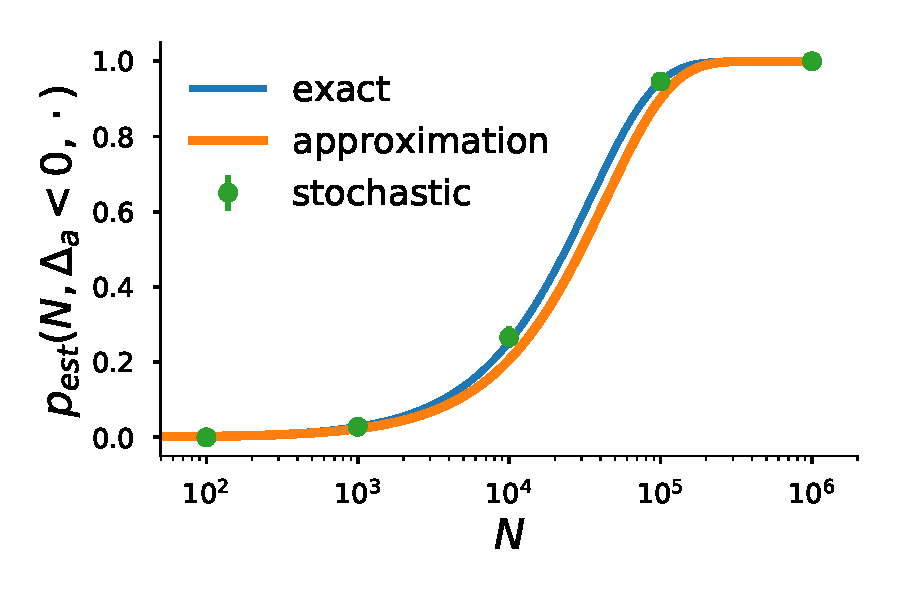
\includegraphics[width=1\textwidth]{DeleteriousTauLeapPlot.pdf}
\caption{Plot of the probability of survival of a population as a function of the initial population size of wildtype cells. The continuous lines represent the exact result \eqref{survprobw} while the dashed lines represent the approximation \eqref{pestthirdcase}.}
\label{DeleteriousPlot}
\end{figure}
%%%%%%%%%%%%%%%%%%%%%%%%%%%%%%%%%%%%%%%%%%%%%%%%%%%%%%%%%%%%%%%%%%%%
\section{Second case: $4\lambda_avp_m>\left(\lambda_a-\mu_a-v\right)^2$}
If we assume that  $4\lambda_avp_m>\left(\lambda_a-\mu_a-v\right)^2$ then we write:
\begin{equation}
p_a=\frac{\lambda_a-\mu_a-v+2\sqrt{\lambda_a vp_m}\left(1+\frac{\left(\lambda_a-\mu_a-v\right)^2}{4\lambda_avp_m}\right)^{\frac12}}{2\lambda_a}
\end{equation}
and using the following Taylor series expansion:
\begin{align*}
\left(1+\frac{\left(\lambda_a-\mu_a-v\right)^2}{4\lambda_avp_m}\right)^{\frac{1}{2}}=1+\frac{\left(\lambda_a-\mu_a-v\right)^2}{8\lambda_avp_m}+\cdots
\end{align*}
we obtain:
\begin{align*}
p_a&\approx\frac{\lambda_a-\mu_a-v+2\sqrt{\lambda_a vp_m}\left[1+\frac{\left(\lambda_a-\mu_a-v\right)^2}{8\lambda_avp_m}\right]}{2\lambda_a}\\
&=\frac{\lambda_a-\mu_a-v+2\sqrt{\lambda_a vp_m}+\frac{\left(\lambda_a-\mu_a-v\right)^2}{4\sqrt{\lambda_avp_m}}}{2\lambda_a}\\
&=\frac{\left(\lambda_a-\mu_a-v+2\sqrt{\lambda_avp_m}\right)^2+4\lambda_avp_m}{8\lambda_a\sqrt{\lambda_avp_m}}\\
&=\frac{4\lambda_avp_m+4\lambda_avp_m\left(1+\frac{\lambda_a-\mu_a-v}{2\sqrt{\lambda_avp_m}}\right)^2}{8\lambda_a\sqrt{\lambda_avp_m}}\\
&=\frac{1}{2\lambda_a}\left(\lambda_a-\mu_a-v+2\sqrt{\lambda_avp_m}\right)
\end{align*}
%In the last line of the above we have used the following inequalities:
%\begin{align*}
%\lambda_a-\mu_a,\,v,\,\frac{\left(\lambda_a-\mu_a-v\right)^2}{4\sqrt{\lambda_avp_m}}\ll1.
%\end{align*}
As a result, we have from \eqref{survprobwinitial} the probability of rescue of a population starting from one wildtype individual:
\begin{align*}
p_w&\approx-\frac{1}{\lambda_w-\mu_w-u-v}\left[v\frac{\lambda_m-\mu_m}{\lambda_m}+\frac{u}{2\lambda_a}\left(\lambda_a-\mu_a-v+2\sqrt{\lambda_avp_m}\right)\right]\\
&=-\frac{1}{\lambda_w-\mu_w-u-v}\left[v\frac{\lambda_m-\mu_m}{\lambda_m}+\frac{u}{2\lambda_a}\left(\lambda_a-\mu_a-v\right)+u\sqrt{\frac{v\left(\lambda_m-\mu_m\right)}{\lambda_a\lambda_m}}\right]\\
&=-\frac{1}{\Delta_w-u-v}\left[v\frac{\Delta_m}{\lambda_m}+\frac{u\left(\Delta_a-v\right)}{2\lambda_a}+u\sqrt{\frac{v\Delta_m}{\lambda_a\lambda_m}}\right],
\end{align*}
where in the last line we have used the notations defined in \eqref{notationalconv}.

Given an initial population consisting of $N$ wildtype cancer cells, the probability that the population will survive is given by: 
\begin{align}\label{pestthirdcase}
p_{est}=1-\left(1-p_w\right)^N\approx 1-\e^{-Np_w}=1-\exp\left[\frac{N}{\Delta_w-u-v}\left(v\frac{\Delta_m}{\lambda_m}+\frac{u\left(\Delta_a-v\right)}{2\lambda_a}+u\sqrt{\frac{v\Delta_m}{\lambda_a\lambda_m}}\right)\right],
\end{align}
which we plot in Figure \ref{DeleteriousPlot} where we compare with numerical simulations and the exact result \eqref{survprobw}.

\begin{align}
\Delta_a^*=2vp_m+v+2\sqrt{vp_m\left(vp_m+\mu_a+v\right)}
\end{align}

The probability of evolutionary rescue is given by:
\begin{equation}
p_{est}\sim\left\{
  \begin{array}{@{}ll@{}}
  1-\exp\left[\frac{N}{\Delta_w-u-v}\left(v\frac{\Delta_m}{\lambda_m}+\frac{u\left(\Delta_a-v\right)}{2\lambda_a}+u\sqrt{\frac{v\Delta_m}{\lambda_a\lambda_m}}\right)\right],\quad\text{if }4\lambda_avp_m>\left(\Delta_a-v\right)^2,\\
   1-\exp\left[\frac{v\Delta_mN}{\lambda_m\Delta_w}\left(1-\frac{u}{\Delta_a}\right)\right],\quad\text{if }\Delta_a<0\quad\text{and}\quad4\lambda_avp_m<\left(\Delta_a-v\right)^2,\\
   1-\exp\left[\frac{N}{\Delta_w}\left(\frac{v\Delta_a}{\lambda_a}+\frac{uv\Delta_m}{\lambda_m\Delta_a}+\frac{v\Delta_m}{\lambda_m}\right)\right],\quad\text{if }\Delta_a>0\quad\text{and}\quad4\lambda_avp_m<\left(\Delta_a-v\right)^2.
  \end{array}\right.
\end{equation}
%%%%%%%%%%%%%%%%%%%%%%%%%%%%%%%%%%%%%%%%%%%%%%%%%%%%%%%%%%%%
\section{Logistic}
We want to have birth and death rates which depends on the population size of wildtype $w$, aneuploidy $a$ and mutant $m$ cells:
\begin{align*}
&\lambda_w'=\lambda_w,\quad\mu_w'=\mu_w\\
&\lambda_a'=C_1+\lambda_a\left(1-\frac{w+a+m}{K}\right),\quad \mu_a'=C_1\\
&\lambda_m'=C_2+\lambda_m\left(1-\frac{w+a+m}{K}\right),\quad \mu_m'=C_2
\end{align*}
where $C_1, C_2>0$ are constants.
%%%%%%%%%%%%%%%%%%%%%%%%%%%%%%%%%%%%%%%%%%%%%%%%%%%%%%%%%%%%
\section{Standing genetic variation}
Until now we have assumed that the initial population of cells consisted entirely of wildtype cells. We modify this assumtion such that the initial population includes a fraction $f$ of cells with aneuploidy. The probability of evolutionary rescue by the cells with aneuploidy from the initial population is:
\begin{equation*}
p_{old}=1-\left(1-p_a\right)^{fN}\approx 1-\e^{-fNp_a}.
\end{equation*}
The total probability of evolutionary rescue is given by:
\begin{align}\nonumber
p_{total}&=p_{new}+\left(1-p_{new}\right)p_{old}\\
&=1-\e^{-\left[\left(1-f\right)p_w+fp_a\right]N}.
\end{align}
The fraction of the cases in which the population is rescued by the standing genetic variation is given by:
\begin{align*}
F\left(f\right)=\frac{p_{old}}{p_{total}}=\frac{ 1-\e^{-fNp_a}}{1-\e^{-\left[\left(1-f\right)p_w+fp_a\right]N}}.
\end{align*}
We let $F=\frac{1}{2}$ and we obtain:
\begin{equation}\label{halfeqstandvar}
f^*\approx\frac{p_w}{p_w+p_a},
\end{equation}
wher we have used the expansion $\e^x\approx 1+x$.
We plot $F$ and $f^*$ in Figure \ref{FractionPlot}.

\section{Mean time}
%%%
\begin{figure}[!t]
 \vspace*{1\baselineskip}
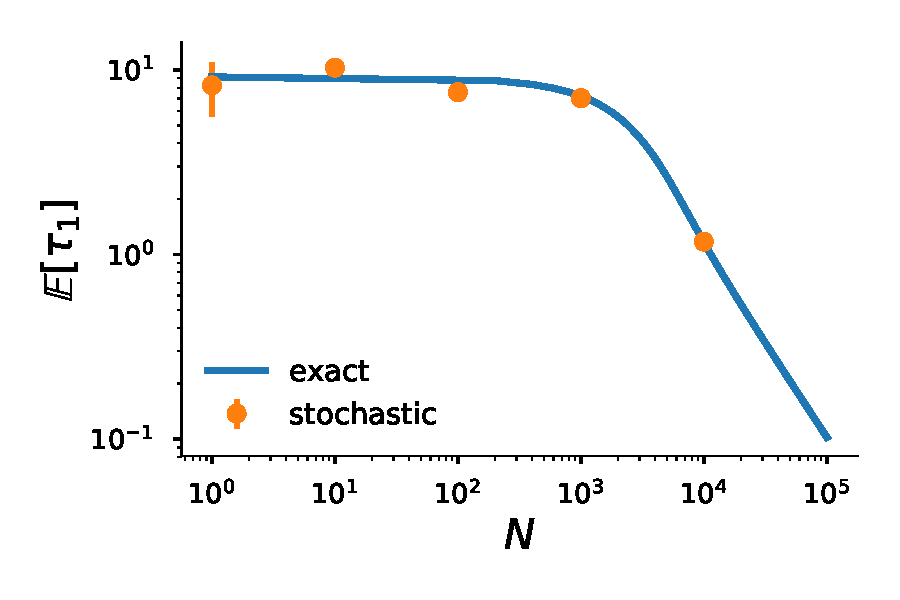
\includegraphics[width=1\textwidth]{MeanTimeGrowthAneuploidyPlot.pdf}
\caption{}
\label{MeanTimeGrowthAneuploidyPlot}
\end{figure}
%%%

\begin{align}
\tau=\tau_1+\tau_2
\end{align}
inhomogeneus Poisson process
\begin{align}
\tau_1\sim \text{Poisson}\left(\frac{1}{up_aW\left(t\right)}\right)
\end{align}
where 
\begin{equation}
W\left(t\right)=W_0\e^{\Delta_wt}
\end{equation}
\begin{align}
f\left(\tau_1\right)=R\left(\tau_1\right)\e^{-\int_0^{\tau_1} R(t)\d t}
\end{align}
\begin{align*}
P\left(\tau_1<t\right)&=P\left(\tau_1<t|M\left(t\rightarrow\infty\right)\neq0\right)P\left(M\left(t\rightarrow\infty\right)\neq0\right)\\
&+P\left(\tau_1<t|M\left(t\rightarrow\infty\right)=0\right)P\left(M\left(t\rightarrow\infty\right)=0\right)\\
P\left(\tau_1<t\right)&=P\left(\tau_1<t|M\left(t\rightarrow\infty\right)\neq0\right)P\left(M\left(t\rightarrow\infty\right)\neq0\right)
\end{align*}
where we used
\begin{align*}
P\left(\tau_1<t|M\left(t\rightarrow\infty\right)=0\right)=0
\end{align*}
\begin{align}
P\left(\tau_1<t|M\left(t\rightarrow\infty\right)\neq0\right)=\frac{P\left(\tau_1<t\right)}{1-\left(1-p_w\right)^N}
\end{align}
where we have used
\begin{equation}
P\left(M\left(t\rightarrow\infty\right)\neq0\right)=1-\left(1-p_w\right)^N
\end{equation}
\begin{align}
f\left(\tau_1|M\left(t\rightarrow\infty\right)\neq0\right)=\frac{R\left(\tau_1\right)\e^{-\int_0^{\tau_1} R(t)\d t}}{1-\left(1-p_w\right)^N}
\end{align}
\begin{align}
\mathbb{E}\left[\tau_1\right]&=\frac{\int_0^\infty\e^{-\int_0^\tau R(t)\d t}\d\tau}{1-\left(1-p_w\right)^N}\\
&=\frac{\int_0^\infty\e^{-uNp_a\frac{\e^{\Delta_w\tau}-1}{\Delta_w}}\,\d\tau}{1-\left(1-p_w\right)^N}
\end{align}
\begin{align}
P_2\left(\tau_2\right)&=\int_0^\infty \d w P\left(W_l=w\right)\left[1-\e^{-vp_mW_l\left(\tau_2\right)}\right]\\
&=1-\mathbb{E}\left[\e^{-vp_mW_l\left(\tau_2\right)}\right]
\end{align}
\begin{align}
a_\pm=\frac{2-\delta-y\pm\sqrt{\left(\delta+y\right)^2-4y}}{2\left(1-\delta\right)}
\end{align}
\begin{align}
P_2\left(\tau_2\right)=\frac{\left(a_+-1\right)\left(1-a_-\right)\left(1-\e^{\left[-\left(1-\delta\right)\left(a_+-a_-\right)t\right]}\right)}{a_+-1+\left(1-a_-\right)\e^{\left[-\left(1-\delta\right)\left(a_+-a_-\right)t\right]}}
\end{align}
with $y=vp_m$ in $a_\pm$.
\begin{align}
\mathbb{E}\left[\tau_2\right]=\int_0^\infty\left(1-\frac{P_2\left(t\right)}{p_m}\right)\d t
\end{align}
\section{Discussion}



\begin{figure}[!t]
 \vspace*{1\baselineskip}
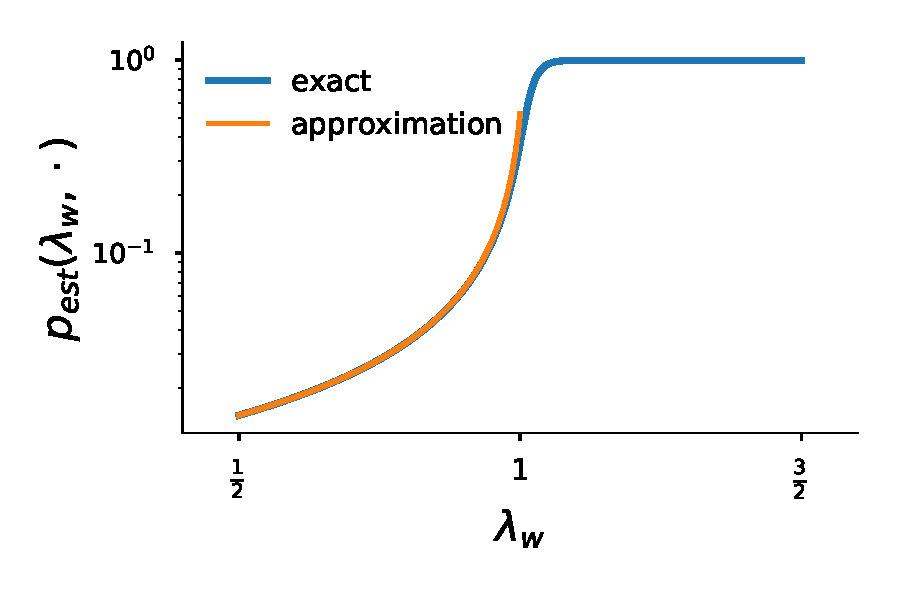
\includegraphics[width=1\textwidth]{SurvPlot.pdf}
\caption{Plot of the probability of survival of a population as a function of the proliferation rate of the wildtype cells. The blue line represents the exact solution \eqref{survprobw} and the orange line line represents the approximation \eqref{survprobwapprox}. Here the population initially consists of $N$ wildtype cells and for the simulations we have chosen the following parameters: $N=75, \lambda_a=1+10^{-2},\lambda_m=1+10^{-3},\mu_w=1,\mu_a=1,\mu_m=1.$}
\label{SurvPlot}
\end{figure}

\begin{figure}[!t]
 \vspace*{1\baselineskip}
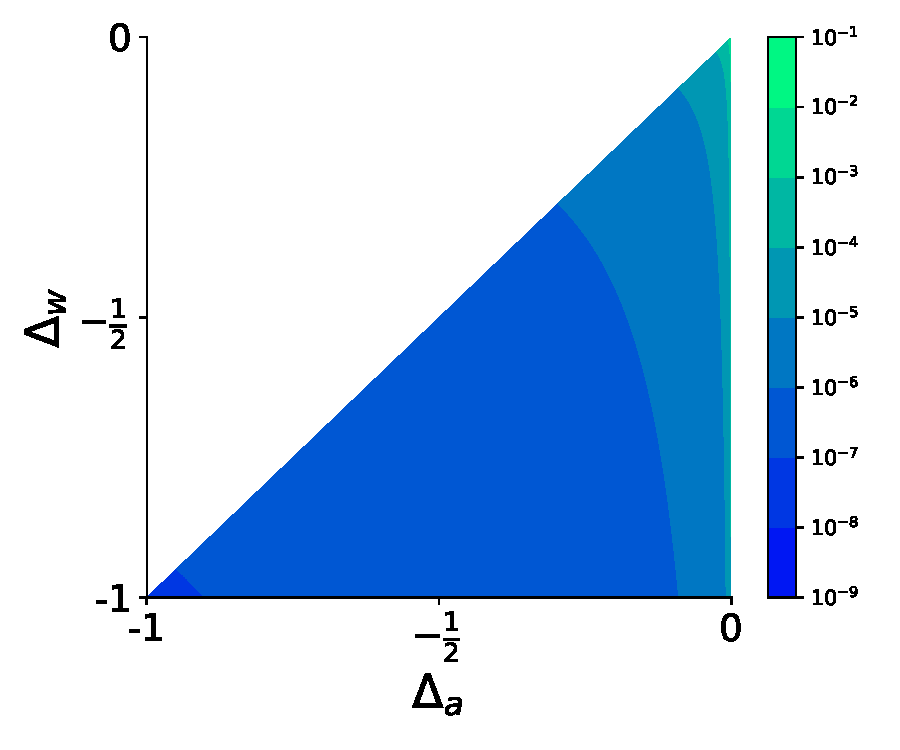
\includegraphics[width=1\textwidth]{HeatMap_p_est.pdf}
\caption{Contours of the survival probability of an initial population consisting of $10^{3}$ wildtype cells as a function of the
   parameters $\Delta_w=\lambda_w-\mu_w$ and $\Delta_a=\lambda_a-\mu_a$.}
\label{SurvHeatMapPlot}
\end{figure}

\begin{figure}[!t]
 \vspace*{1\baselineskip}
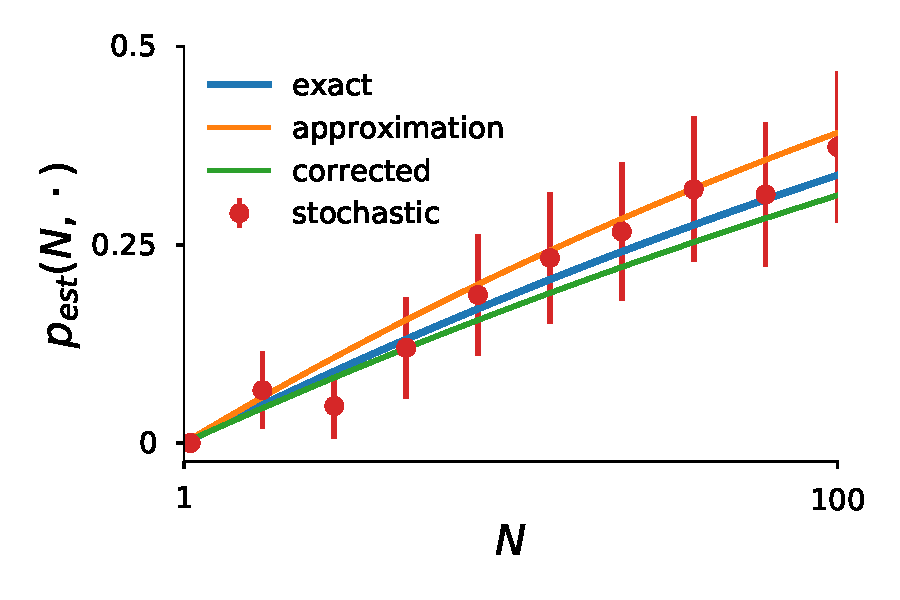
\includegraphics[width=1\textwidth]{SurvPlotNData.pdf}
\caption{Plot of the probability of survival of a population as a function of the initial population size of wildtype cells. The blue line represents the exact solution \eqref{survprobw}, the orange line line represents the approximation \eqref{survprobwapprox}, the green line represents the first order correction \eqref{survprobwapproxcorrected} and the red dots represents stochastic simulations. For the simulations we have chosen the following parameters: $\lambda_w=1-10^{-2}, \lambda_a=1+10^{-2},\lambda_m=1+10^{-1},\mu_w=1,\mu_a=1,\mu_m=1.$}
\label{SurvPlotNData}
\end{figure}

\begin{figure}[!t]
 \vspace*{1\baselineskip}
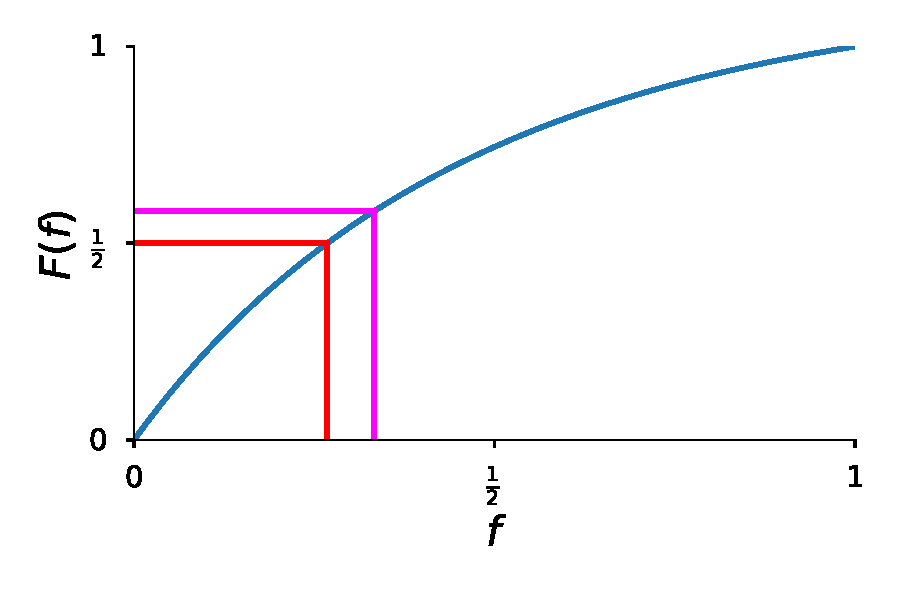
\includegraphics[width=1\textwidth]{FractionPlot.pdf}
\caption{Plot of the fraction of the cases the population is rescue by standing genetic variation as a function of the fraction of initial cells which are aneuploid. The red vertical line highlights the the value of $f$ for which half the times the population is rescues by aneuploid cells while the pink line is our approximation \eqref{halfeqstandvar}. For this plot we have chosen the following parameters: $N=10^3, \lambda_w=1-10^{-2}, \lambda_a=1-10^{-4},\lambda_m=1+10^{-1},\mu_w=1,\mu_a=1,\mu_m=1.$}
\label{FractionPlot}
\end{figure}

\bibliographystyle{unsrt}
\bibliography{evo2022}

\appendix

\section{Gillespie algorithm}
\begin{subequations}
\begin{flalign}
(+1,0,0)&:\quad \lambda_ww_t,\\
(-1,0,0)&:\quad \mu_ww_t,\\
(-1,+1,0)&:\quad uw_t,\\
(-1,0,+1)&:\quad vw_t,\\
(0,+1,0)&:\quad \lambda_aa_t,\\
(0,-1,0)&:\quad \mu_aa_t,\\
(0,-1,+1)&:\quad va_t,\\
(0,0,+1)&:\quad \lambda_am_t,\\
(0,0,-1)&:\quad \mu_am_t.
\end{flalign}
\end{subequations}

\section{Survival probability of a mutant lineage}\label{AppendixSurvLin}
The infinitesimal transition probabilities for the simple birth and death process:
\begin{align*}
p_{i+j,i}\left(\Delta t\right)=\left\{
  \begin{array}{@{}ll@{}}
  \mu i\Delta t+o\left(\Delta t\right),\quad j=-1 \\
  \lambda i\Delta t+o\left(\Delta t\right),\quad j=1 \\
    1-\left(\lambda+\mu\right) i\Delta t+o\left(\Delta t\right),\quad j=0 \\
   o\left(\Delta t\right),\quad j\neq-1,0,1.
  \end{array}\right.
\end{align*}
The forward Kolmogorov differential equations are:
\begin{subequations}
\label{KolmeqSurv}
\begin{flalign}
\frac{dp_i\left(t\right)}{dt}&=\lambda\left(i-1\right)p_{i-1}\left(t\right)+\mu\left(i+1\right)p_{i+1}\left(t\right)-\left(\lambda+\mu\right)ip_i\left(t\right),\\
\frac{dp_0\left(t\right)}{dt}&=\mu p_1\left(t\right),
\end{flalign}
\end{subequations}
for $i=1,2,\dots$ with initial conditions $p_i\left(0\right)=\delta_{iN}$.

The probability generating function is defined as:
\begin{equation*}
\mathcal{P}\left(z,t\right)=\sum_{i=0}^\infty p_i\left(t\right)z^i
\end{equation*}
which we obtain by multiplying \eqref{KolmeqSurv} by $z^i$ and summing over $i$:
\begin{align*}
\mathcal{P}\left(z,t\right)=\left\{
  \begin{array}{@{}ll@{}}
  \left(\frac{\e^{t\left(\mu-\lambda\right)}\left(\lambda z-\mu\right)-\mu\left(z-1\right)}{\e^{t\left(\mu-\lambda\right)}\left(\lambda z-\mu\right)-\lambda\left(z-1\right)}\right)^N,\quad \text{if }\lambda\neq\mu, \\
  \left(\frac{1-\left(\lambda t-1\right)\left(z-1\right)}{1-\lambda t\left(z-1\right)}\right)^N,\quad \text{if }\lambda=\mu.
  \end{array}\right.
\end{align*}
The probability $p_i$ can be obtained from the probability generating function as:
\begin{equation*}
p_i\left(t\right)=\left.\frac{1}{i!}\frac{\partial^i\mathcal{P}}{\partial z^i}\right|_{z=0},
\end{equation*}
and the probability of extinction is given by:
\begin{align*}
p_0\left(t\right)=\left\{
  \begin{array}{@{}ll@{}}
  \left(\frac{\mu-\mu\e^{\left(\mu-\lambda\right)t}}{\lambda-\mu\e^{\left(\mu-\lambda\right)t}}\right)^N,\quad \text{if }\lambda\neq\mu, \\
  \left(\frac{\lambda t}{1+\lambda t}\right)^N,\quad \text{if }\lambda=\mu.
  \end{array}\right.
\end{align*}
When $t\rightarrow\infty$ the extinction probability has the following expression:
\begin{align*}
p_0\left(\infty\right)=\lim_{t\rightarrow\infty}p_0\left(t\right)=\left\{
  \begin{array}{@{}ll@{}}
  1,\quad \text{if }\lambda\leq\mu, \\
  \left(\frac{\mu}{\lambda}\right)^N,\quad \text{if }\lambda>\mu.
  \end{array}\right.
\end{align*}
\end{document}